
\makeatletter
\def\input@path{{../../}}
\makeatother
\documentclass[../../main.tex]{subfiles}

\graphicspath{
	{../../img/}
	{../img/}
	{img/}
}

\begin{document}

Для определенного интеграла Римана, рассматриваемого на конечном промежутке,
необходимым условием сходимости является ограниченность подынтегральной 
функции.
НИ возникает, если конечный промежуток заменить на $+\infty$.

\section{Несобственный интеграл первого рода (НИ-1)}

Рассмотрим функцию $f(x)$, т.~ч.
$\forall x \in [a, +\infty[ \ \forall A > a \implies f \in R([a, A])$.
В этом случае корректно определена функция
\begin{equation}
    \label{7:1}
    \Phi(A) = \displaystyle\int\limits_a^A f(x)dx,\quad\forall A \geq a
\end{equation}

Если $\exists \ \Phi(+\infty) \in \R$, имеем \emph{сходящийся НИ-1} вида:
\begin{equation}
    \label{7:2}
    \int\limits_a^{+\infty} f(x)dx =
    \lim\limits_{A \to \infty} \int\limits_a^A f(x)dx
\end{equation}

У этого интеграла $\Phi(+\infty)$ берется за значение этого интеграла. Если 
окажется,
что ${\Phi(+\infty) \notin \R}$ или $ \nexists \Phi(+\infty)$, то 
рассматриваемый НИ-1 расходится.
Аналогично определяется НИ-1 вида:
\[\int\limits_{-\infty}^a f(x)dx =
\lim\limits_{B \to \infty} \int\limits_{-B}^a f(x)dx, \]
сходимость и расходимость которого аналогична предыдущему.
Будем также рассматривать \emph{НИ-1 общего вида}:
\[ \int\limits_{-\infty}^{+\infty} f(x)dx =
\lim\limits_{\substack{A \to +\infty \\ B \to +\infty}}
\int\limits_{-B}^A f(x)dx =
\lim\limits_{\substack{A \to +\infty \\ B \to +\infty}}
\left( \int\limits_{-B}^a f(x)dx + \int\limits_a^{A} f(x)dx \right), \]
который сходится $\iff$ сходятся интегралы:
\[ \lim\limits_{B \to +\infty} \int\limits_{-B}^a f(x)dx
= \int\limits_{-\infty}^a f(x)dx \]
\[\lim\limits_{A \to +\infty} \int\limits_a^{A} f(x)dx
= \int\limits_a^{+\infty} f(x)dx \]
Если хотя бы один из них не сходится, то исходный интеграл не сходится.

В общем случае НИ-1 выглядит так:
\[ \int\limits_{-\infty}^{+\infty} f(x)dx  = \int\limits_{-\infty}^a f(x)dx
+ \int\limits_a^{+\infty} f(x)dx.\]

Для простоты ограничимся НИ-1 вида \eqref{7:1}, для остальных результаты будут
аналогичными. Для сходящихся НИ-1 вида \eqref{7:1} подынтегральную функцию 
называют \emph{интегрируемой в несобственном смысле} на $[a, +\infty[$.

Геометрически:

Если $\forall x \geq a \implies f(x) \geq 0$, то учитывая, что в случае 
непрерывной $f(x)$ на $[a, +\infty[$ получаем, что
$\int\limits_a^A f(x)dx = S_{\text{тр.}}$ (площадь криволинейной трапеции). 
Тогда при
$A \to \infty$ получаем, что $\int\limits_a^{+\infty} f(x)dx$~--- площадь 
незамкнутой фигуры, заключенной между $x = a$ и $f(x)$.

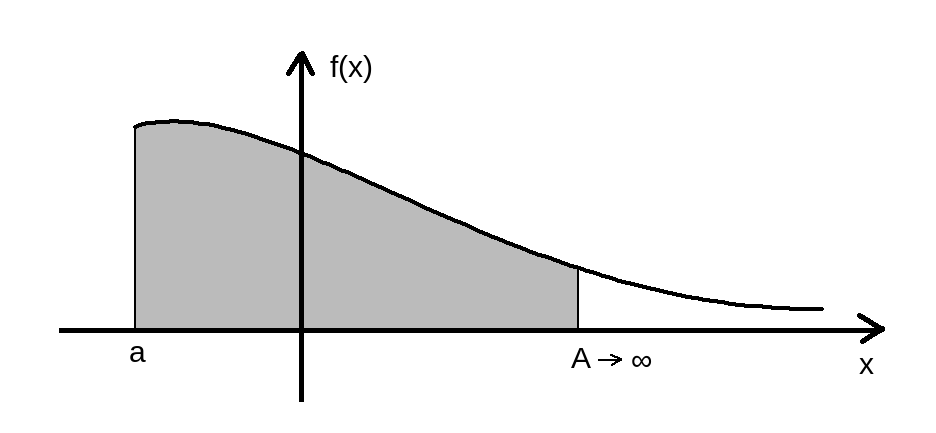
\includegraphics[scale = 0.3]{lec7_1.png}

Из соответствующих свойств интеграла Римана и свойств операций предельного
перехода получаем следующие свойства НИ-1:
\begin{enumerate}
        \item Линейность:
        
        Если сходятся $\displaystyle\int\limits_a^{+\infty} f(x)dx$ и
        $\displaystyle\int\limits_a^{+\infty} g(x)dx$, то \[\forall \alpha, 
        \beta \in \R
        \implies  \exists \int\limits_a^{+\infty} \left( \alpha f(x)
        + \beta g(x) \right)dx = \left( \alpha \int\limits_a^{+\infty}
        f(x)dx + \beta \int\limits_a^{+\infty} g(x)dx \right) \in \R.\]
        \item Аддитивность:
        
        Можно заметить, что если $\displaystyle\int\limits_a^{+\infty} f(x)dx$ 
        сходится, то
        $\forall b>a$ сходится остаток, т.~е.
        $\displaystyle\int\limits_{b>a}^{+\infty} f(x)dx$ сходится. Имеем 
        следующую формулу
        аддитивности НИ-1:
        \[\int\limits_a^{+\infty} f(x)dx = \int\limits_a^b f(x)dx +
        \int\limits_b^{+\infty} f(x)dx \]
        \item Монотонность:
        
        Если $f(x)$, $g(x)$ интегрируемы в несобственном смысле на
        $[a, +\infty[$
        и $f(x) \leq g(x) \ {\forall x \in [a, +\infty[}$, то
        \[\int\limits_a^{+\infty} f(x)dx \leq \int\limits_a^{+\infty} g(x)dx.\]
        В частности, т.~к. $\int\limits_a^{+\infty} 0dx = 0, \ \forall a \in 
        \R$, то получаем свойство неотрицательности НИ-1: \[h(x) \geq 0 \ 
        \forall x \in
        [a, +\infty[ \implies \int\limits_a^{+\infty} h(x)dx \geq 0.\]
        \item Критерий сходимости НИ-1:
        
        Если $f(x) \geq 0, \ \forall x \geq a$, то для сходимости
        $ \int\limits_a^{+\infty} f(x)dx$ необходимо и достаточно, чтобы 
        $\Phi(A) =
        \int\limits_a^{A} f(x)dx$ была ограничена для $\forall A \geq a$.
        \begin{proof}
            Проводится по той же схеме, что и у положительных рядов (числовых).
            Здесь $\Phi(A)$ будет монотонно возрастать $\forall A \geq a$
            в силу монотонности НИ-1, т.~к.
            \[\forall \tilde{A} \geq A \geq a
            \implies \Phi(\tilde{A}) - \Phi(A) =
            \int\limits_a^{\tilde{A}} f(x)dx - \int\limits_a^{A} f(x)dx =
            \int\limits_A^{\tilde{A}} \underbrace{f(x)}_{\geq 0} dx \geq 0 \]
            Используем то, что для монотонного возрастания функции значение
            $\Phi (+\infty) \in \R \iff$ функция ограничена сверху.
        \end{proof}
\end{enumerate}
\section{Условия сходимости НИ-1}
Основные условия сходимости НИ-1 аналогичны условиям сходимости числовых рядов.
Ограничимся формулами.
\begin{thm}[Признак сравнения для сходимости НИ-1]
Если $\forall x \geq a \implies 0 \leq f(x) \leq g(x)$, то из
сходимости $\int\limits_a^{+\infty} g(x)dx$ следует сходимость
$\int\limits_a^{+\infty} f(x)dx$, а из расходимости
$\int\limits_a^{+\infty} f(x)dx \implies$
расходимость $\int\limits_a^{+\infty} g(x)dx$.
\end{thm}
\begin{thm}[Предельный признак сравнения для сходимости НИ-1]
Пусть $\forall x \geq a \implies f(x) > 0$ и $g(x) > 0$, тогда:
\begin{enumerate}
    \item Если $\exists \lim\limits_{x \to +\infty} \dfrac{f(x)}{g(x)} = p
    \in \R$, то в случае $p > 0$ :
    $\int\limits_a^{+\infty} f(x)dx$ и $\int\limits_a^{+\infty} g(x)dx $
    одновременно сходятся или расходятся (имеют один и тот же характер
    сходимости (расходимости)).
    \item Если $\exists \lim\limits_{x \to +\infty} \dfrac{f(x)}{g(x)} = 0,$
    $f(x) = o(g(x)), \ x \to \infty$, то тогда из сходимости
    $\int\limits_a^{+\infty} g(x)dx \implies$ сходимость
    $\int\limits_a^{+\infty} f(x)dx$, а из расходимости
    $\int\limits_a^{+\infty} f(x)dx \implies$ расходимость
    $\int\limits_a^{+\infty} g(x)dx$.
    \item Если $\exists \lim\limits_{x \to +\infty}
    \dfrac{f(x)}{g(x)} = +\infty$
    , то тогда из сходимости
    $\int\limits_a^{+\infty} f(x)dx \implies$ сходимость
    $\int\limits_a^{+\infty} g(x)dx$, а из расходимости
    $\int\limits_a^{+\infty} g(x)dx \implies$ расходимость
    $\int\limits_a^{+\infty} f(x)dx$.
\end{enumerate}
\end{thm}

\begin{crl*}[Степенной признак сравнения для сходимости НИ-1]
\end{crl*}

Если $f(x) \underset{x \to + \infty}{\sim} \dfrac{c}{x^\alpha}$, где
$c = const \neq 0, \alpha \in \R$, то $\displaystyle\int\limits_{a > 
0}^{+\infty} f(x)dx =
\begin{cases}
    \text{сходится}, \ \alpha > 1 \\
    \text{расходится}, \ \alpha \leq 1
\end{cases} $
\begin{proof}
    Следует из того, что
    \[ \int\limits_{a > 0}^{+\infty} \dfrac{dx}{x^\alpha} =
    \begin{cases}
        \left. \dfrac{x^{1 - \alpha}}{1 - \alpha} \right\vert_a^{+\infty},
        & \alpha \neq 1 \implies
        \left[
            \begin{array}{ll}
                \dfrac{1}{\alpha - 1} \in \R \text{} , & \alpha > 1
                \text{ \ --- сходится}\\
                + \infty , & \alpha < 1 \text{ \ --- расходится}
            \end{array}
        \right.
        \\
        \left. \ln x \right\vert_a^{+\infty}, &
        \alpha = 1 \text{\ --- расходится} 
    \end{cases} \]
    расходится при $\alpha \leq 1$.
    Тогда применим первый предельный признак
    сравнения для сходимости НИ-1.
  \end{proof}
    \begin{rem}
        Если $f(x) = o \left(\dfrac{1}{x^\alpha}\right), \ x \to + \infty$, то 
        в случае, когда $\alpha > 1$ получаем, что
        $\displaystyle\int\limits_{a > 0}^{+\infty} f(x)dx$ сходится. Если 
        $\alpha \leq 1$
        --- требуются дополнительные исследования.  
    \end{rem}
\end{document}
